Authentication and authorization are managed using Supabase's built-in authentication services, which provide a secure and robust solution for user management based on \ac{jwt}. The platform supports user registration and login via both email/password credentials and an OAuth provider for Google, as shown in the authentication form in Figure~\ref{FIG:AUTH_FORM}.

\begin{figure}[Login Form]{FIG:AUTH_FORM}{The user authentication form for logging in.}
    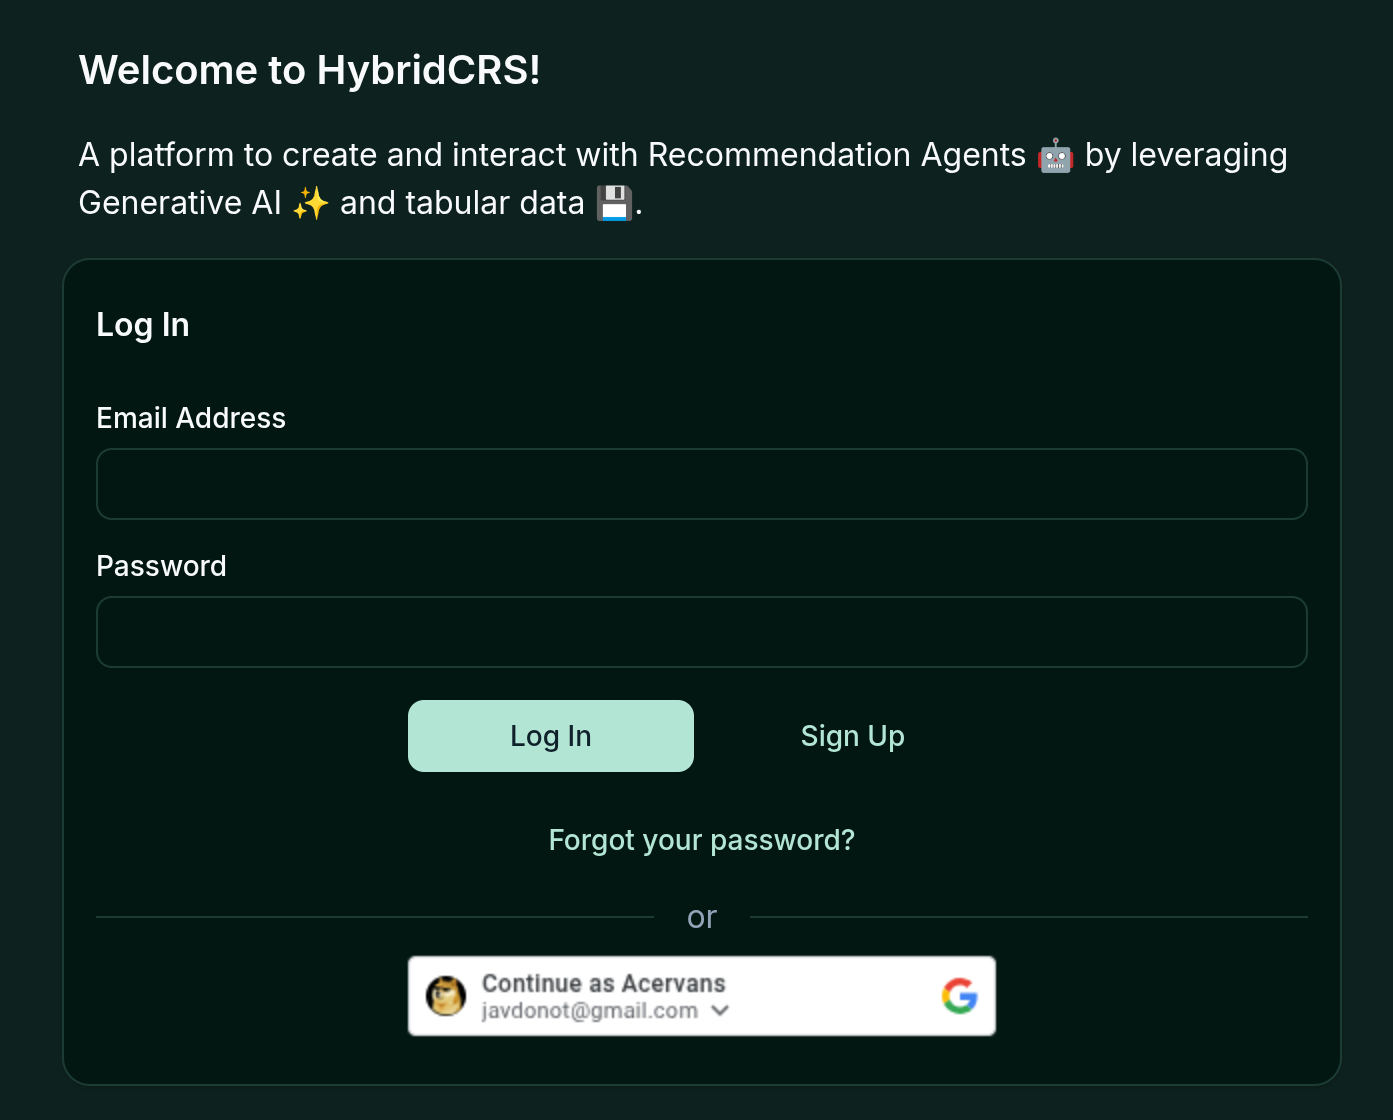
\includegraphics[width=0.7\textwidth]{screenshots/login.png}
\end{figure}

When a user logs in, the Supabase library handles the authentication flow server-side, for better protection of sensitive data such as \acs{api} keys and session tokens. Afterwards, the resulting \acs{jwt} (containing the user's credentials) is securely stored in the browser as a cookie. For every subsequent request to the backend \acs{api}, this \acs{jwt} is retrieved client-side and included in the \texttt{Authorization} header as a bearer token.

The \texttt{SupabaseContext} is convenient in this process by providing the \texttt{getAccessToken} function. This function, used throughout the application before making an \acs{api} call, ensures that a valid and fresh access token is always available. On the backend, a custom FastAPI middleware verifies the token, ensuring that all protected endpoints are only accessible by authenticated users.